\documentclass[10pt,twocolumn,letterpaper]{article}
%% Welcome to Overleaf!
%% If this is your first time using LaTeX, it might be worth going through this brief presentation:
%% https://www.overleaf.com/latex/learn/free-online-introduction-to-latex-part-1

%% Researchers have been using LaTeX for decades to typeset their papers, producing beautiful, crisp documents in the process. By learning LaTeX, you are effectively following in their footsteps, and learning a highly valuable skill!

%% The \usepackage commands below can be thought of as analogous to importing libraries into Python, for instance. We've pre-formatted this for you, so you can skip right ahead to the title below.

%% Language and font encodings
\usepackage[english]{babel}
\usepackage[utf8x]{inputenc}
\usepackage[T1]{fontenc}
\usepackage{amsmath}

%% Sets page size and margins
\usepackage[a4paper,top=3cm,bottom=2cm,left=3cm,right=3cm,marginparwidth=1.75cm]{geometry}

%% Useful packages
\usepackage{amsmath}
\usepackage{graphicx}
\usepackage[colorinlistoftodos]{todonotes}
\usepackage[colorlinks=true, allcolors=blue]{hyperref}
\usepackage{natbib}
\bibliographystyle{unsrt}
%% Title
\title{
		\usefont{OT1}{bch}{b}{n}
		\normalfont \normalsize \textsc{SPH 3U1} \\ [10pt]
		\huge Projectile Motion Lab Report \\
}
\selectlanguage{english}
\usepackage{authblk}
\author[1]{Hanz Nathan Po}

\begin{document}
\maketitle

\section{Objective}
The objective of this lab is to apply kinematics concepts and equations to projectile motion, including uniform horizontal motion, as well as nonuniform vertical motion.

\section{Introduction}
Projectile motion is described as the motion of an object with only the force of gravity affecting it while in motion. Its motion can be resolved to a uniform horizontal component, and a nonuniform vertical component. For the purposes of this lab, factors such as air resistance are negligible and are not taken into account. All calculations are made using SI base units (metres, seconds, etc).

The horizontal component of the object's motion can be described using the following equation
\begin{equation}
    \overrightarrow{\Delta d}_{x}=\overrightarrow{v}_{x}\Delta t
\end{equation}
where \(\overrightarrow{\Delta d}_{x}\) is the horizontal displacement of the object, \(\overrightarrow{v}_{x}\) is the horizontal velocity of the object, and \(\Delta t\) is the amount of time the object is in a state of projectile motion. Calculating any one of these values from any of the other two is a relatively straightforward task due to the uniform nature of the object's horizontal motion. 

On the other hand, the vertical component of the object's motion is nonuniform, with the force of gravity accelerating uniformly it at approximately \(9.8 m/s^2\) towards the centre of the Earth, represented as \(g\). Therefore, the object's vertical motion above its starting point can be described as
\begin{equation}
    \overrightarrow{\Delta d}_{y}=\overrightarrow{v_{iy}}\Delta t+\frac{1}{2}\overrightarrow{g}\Delta t^2
\end{equation}
where \(\overrightarrow{\Delta d}_{y}\) is the vertical displacement of the object above its starting point, \(\overrightarrow{v}_{iy}\) is the initial vertical velocity of the projectile, \(\Delta t\) is the change in time since the object started its motion, and, as mentioned earlier \(g\) is approximately the force of gravity at sea level, or \(9.8 m/s^2\) towards the centre of the Earth. Much like the previous equation, if one of these values is unknown, it can be solved for using algebra. 

When making calculations for projectiles, both the \(\Delta t\) must be equal to one another. Failing to ensure that they are equal can cause inaccurate calculations.

Other equations can also be used to represent the nonuniform vertical motion of the projectile. They can be especially useful in situations where it is necessary to solve for an unknown.
\begin{equation}
    \overrightarrow{\Delta d}_{y}=(\frac{\overrightarrow{v_{fy}}+\overrightarrow{v_{iy}}}{2})\Delta t
\end{equation}
All variables are the same as the previous equation, except the addition of \(V_{fy}\), which represents the final vertical velocity of the projectile. If the final displacement of the object relative to its starting position is equal to zero, the value of \(V_{fy}\) is equal to \(-V_{iy}\).
The following equations use the same variables, and can also be useful to describe different aspects of the vertical nonuniform motion.
\begin{equation}
    \overrightarrow{\Delta d}_{y}=\overrightarrow{v_{fy}}\Delta t-\frac{1}{2}\overrightarrow{g}\Delta t^2
\end{equation}
\begin{equation}
    \overrightarrow{v_{fy}^2}=\overrightarrow{v_{iy}^2}+2\overrightarrow{g} \overrightarrow{\Delta d}
\end{equation}
\begin{equation}
    \Delta t=\frac{\overrightarrow{v_{fy}}-\overrightarrow{v_{iy}}}{\overrightarrow{g}}
\end{equation}


\section{Materials \& Procedure}

In order to perform this experiment, a ball, a video recording device, and a few friends are necessary. To start, get two people to stand a reasonable distance apart from each other. Give the ball to one of the people. Get a third person to hold an object with a fixed length, preferably a metre. A fourth person is to record from a position in which all three other people are clearly visible. The person with the ball is to then throw it towards the other person, preferably allowing the ball to reach a significant height in the process. Using a software such as Logger Pro, plot data from the video and prepare it for analysis. 

\begin{figure}
  \centering
  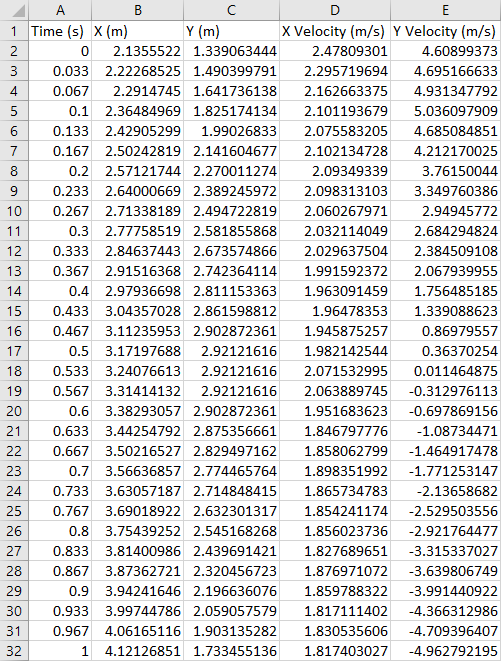
\includegraphics[width=0.5\textwidth]{figures/EXCEL_Jr3LyFPYsU.png}
  \caption{Table of values generated from recording of projectile motion}
\end{figure}

\section{Observations}

\begin{figure}
  \centering
  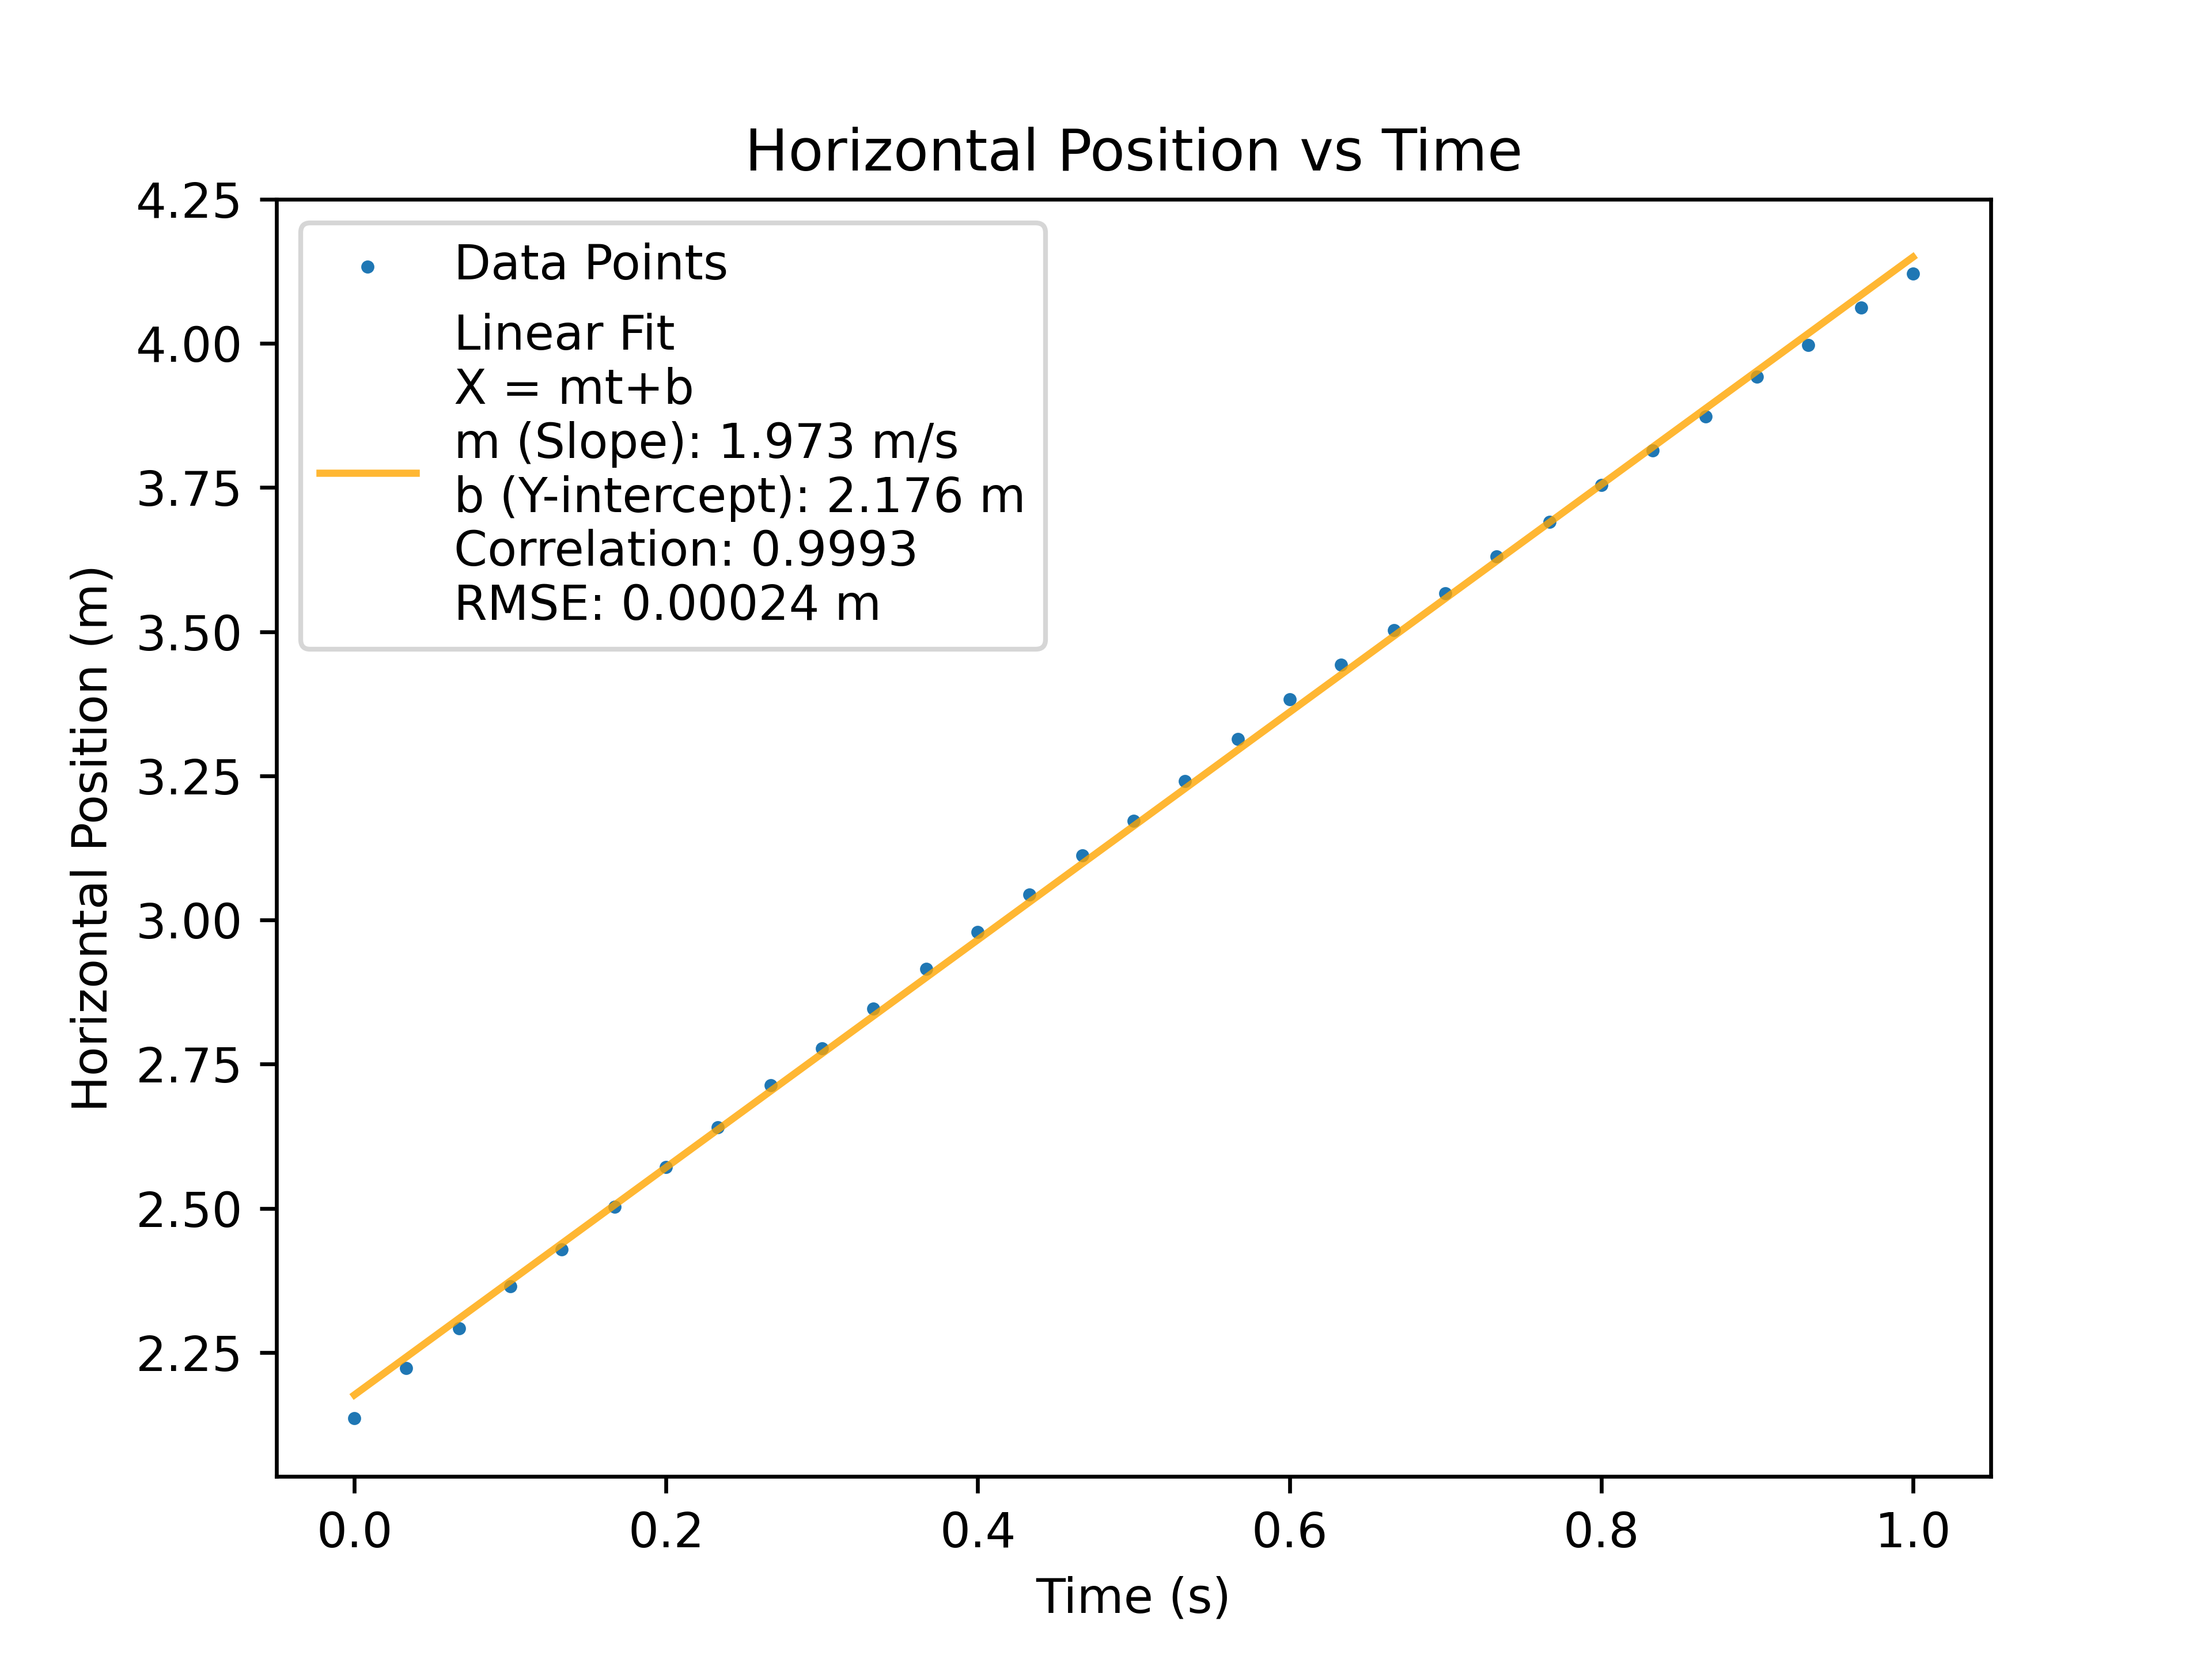
\includegraphics[width=0.5\textwidth]{figures/distance_vs_time.png}
  \caption{Graph of the vertical position over time. A curve fit was created based on the data plotted from the experiment}
\end{figure}

As expected, due to the fact that there is no force acting on the object horizontally, in figure 2, we can clearly observe that the horizontal motion of the object is uniform, as there is no horizontal acceleration. The slope of the generated line tells us the velocity of the object, because it shows the change in displacement over time, or, in metric, \(1.975 m/s\), so for every second that passes, the object travels \(1.975m\). Calculating the displacement at a given time is straightforward by using the uniform equation mentioned earlier.

\begin{figure}
  \centering
  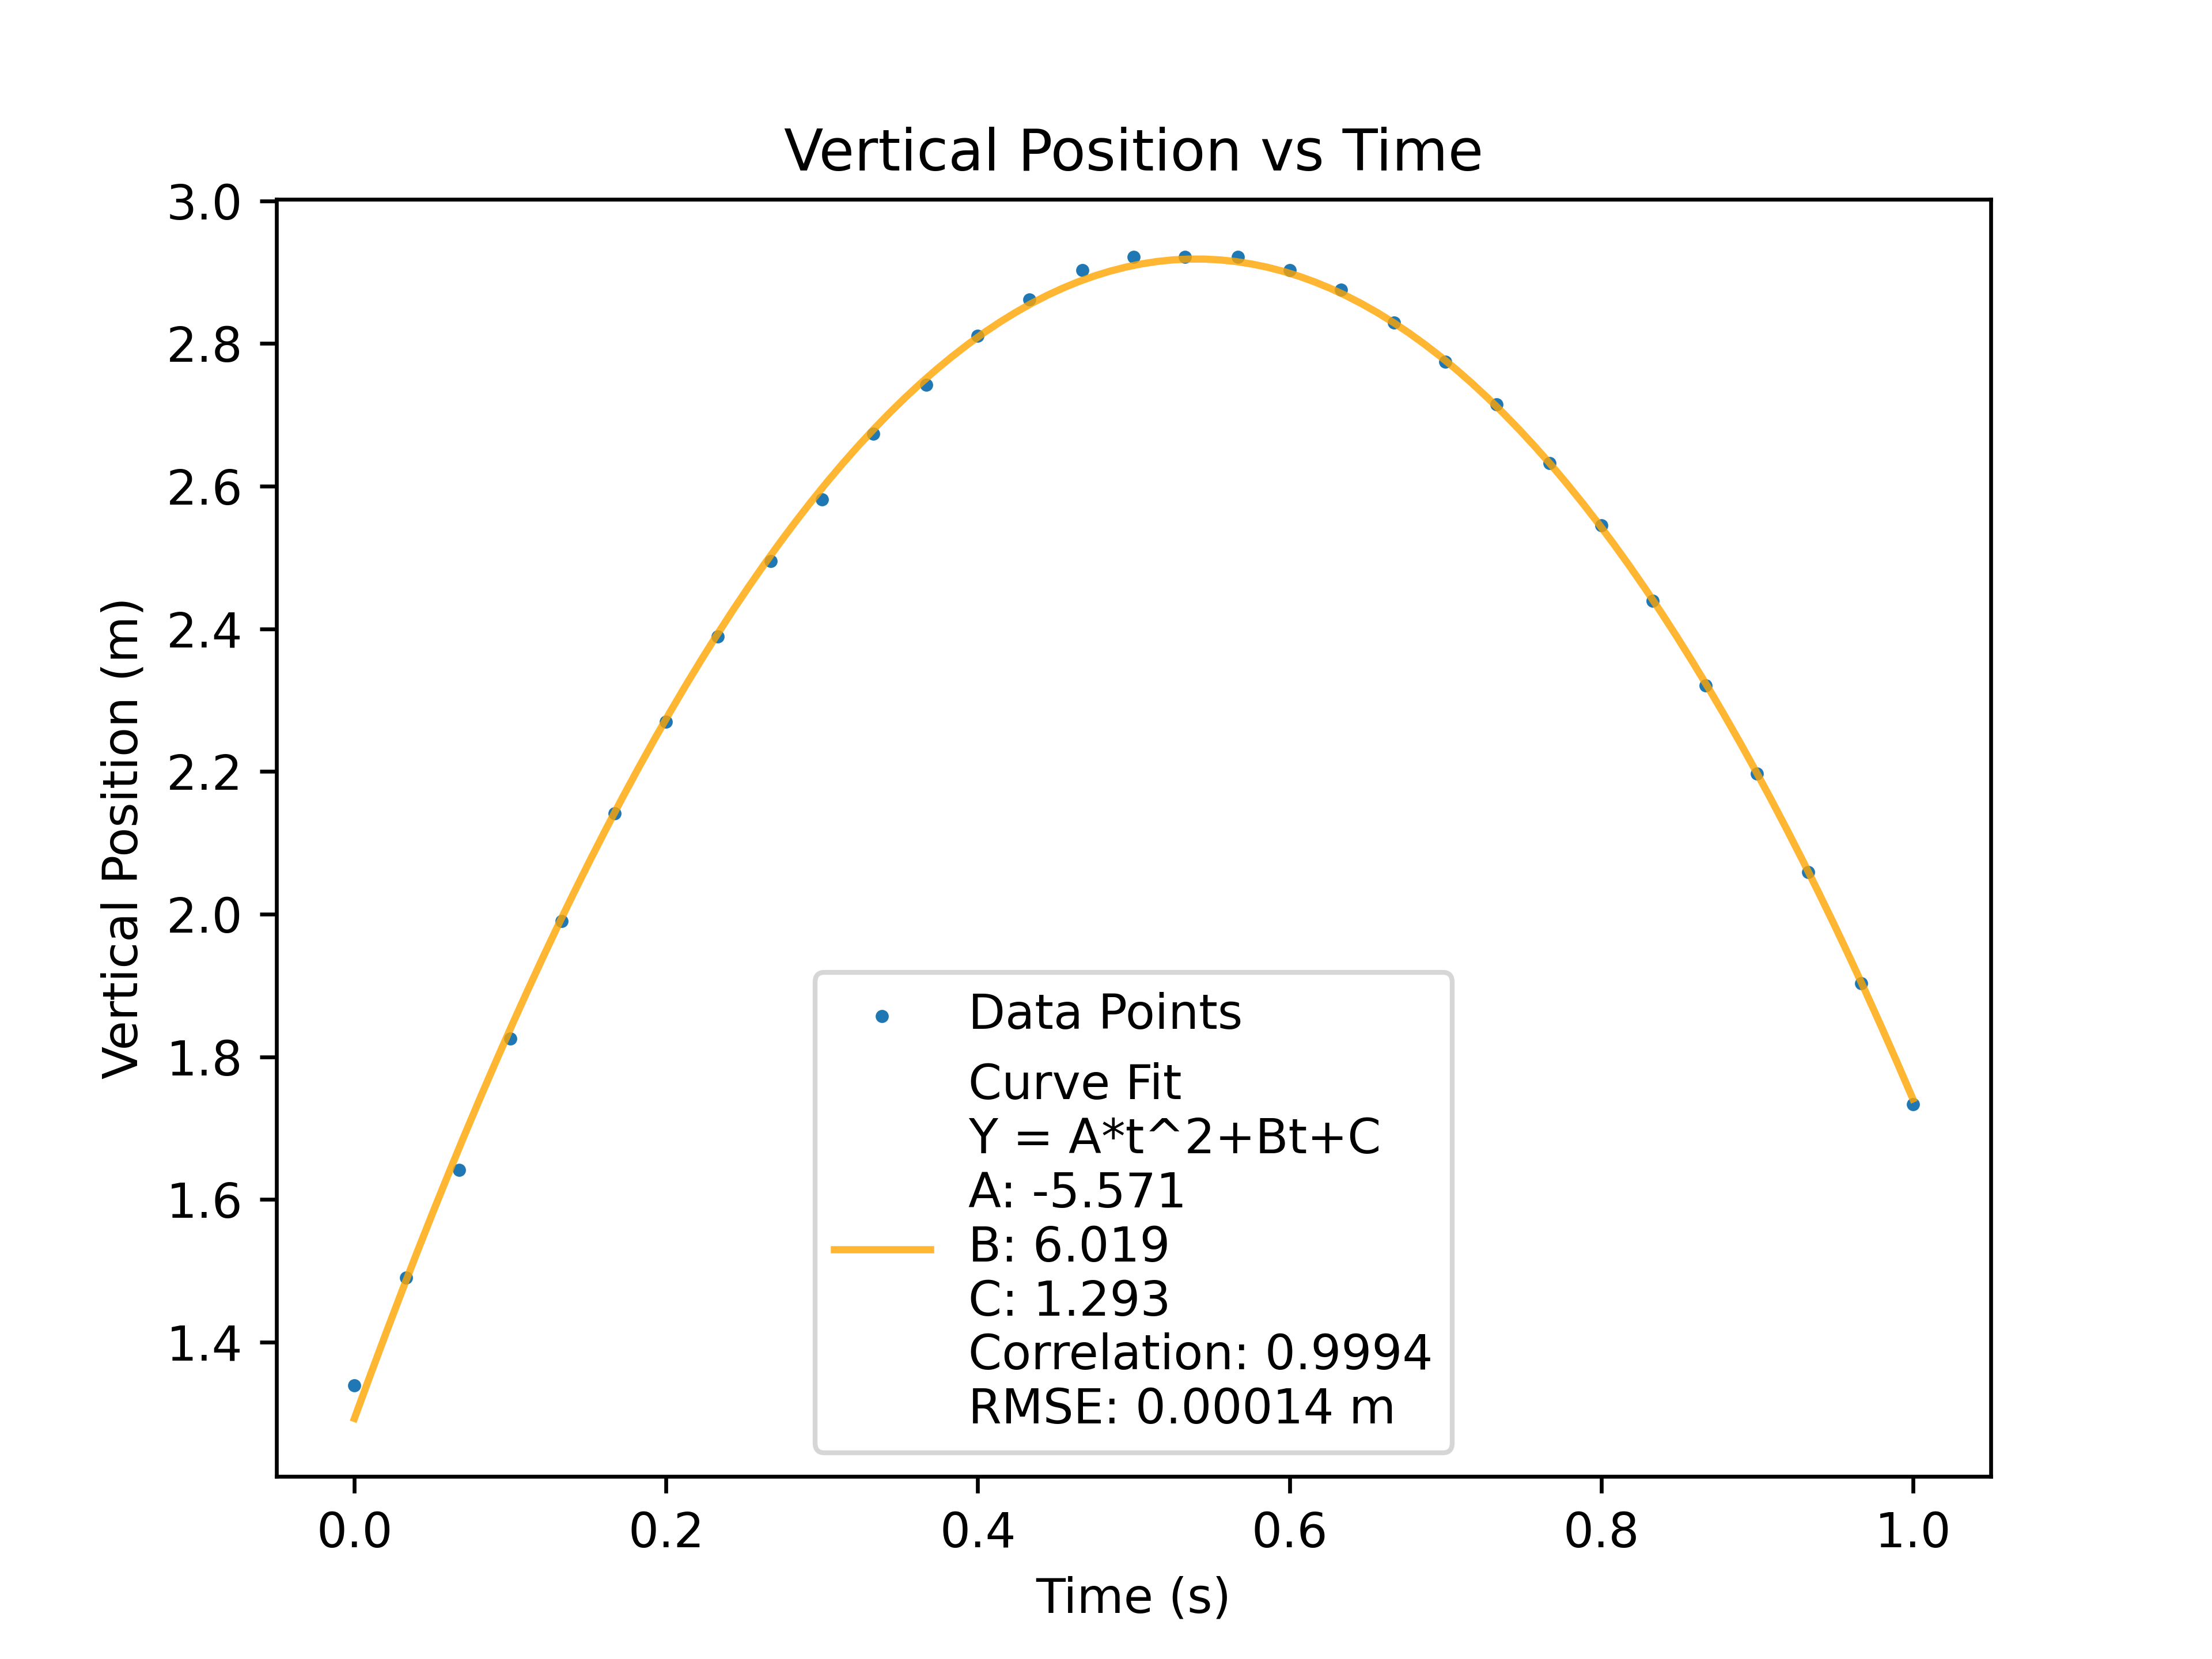
\includegraphics[width=0.5\textwidth]{figures/height_vs_time.png}
  \caption{Graph of the horizontal position over time. A linear fit was created based on the plotted data}
\end{figure}

Since gravity is acting on the object vertically, its velocity is accelerated downward throughout its entire motion. This results in a vertical motion of a parabolic nature, as can be clearly observed in figure 3. To calculate the object's maximum height, we can find the time at which the object is at its maximum height, then plug it into the parabola generated by Logger Pro, which will give us its displacement above the start position.

We know that the instantaneous velocity of the object at its peak has to be zero, we can solve for the time at which the object is at its peak by finding the derivative of the parabola, then setting it equal to zero. The derivative can be found by using the power rule. 

\begin{align}
    \nonumber\frac{d}{dx}(-5.571\Delta t^2+6.019\Delta t+1.293)\\
    \nonumber=-(2)5.571\Delta t+6.019\\
    \nonumber=-11.142\Delta t+6.019
\end{align}

Now we can simply set it equal to zero to find the time at which the object will reach its maximum height. 

\begin{align}
\nonumber-11.142\Delta t+6.019=0\\
\nonumber-11.142\Delta t=-6.019\\
\nonumber\Delta t=\frac{-6.019}{-11.142}\\
\nonumber\Delta t\approx 0.54s
\end{align}

From this, we know that the object will reach its maximum height at around 0.54 seconds. Now we can solve for \(\overrightarrow{\Delta d_{y}}\) by plugging this value into the equation of the parabola. 

\begin{align}
\nonumber\overrightarrow{\Delta d}_{y}=-5.571\Delta t^2+6.019\Delta t+1.293\\
\nonumber\overrightarrow{\Delta d}_{y}=-5.571(0.54)^2+6.019(0.54)+1.293\\
\nonumber\overrightarrow{\Delta d}_{y}\approx2.919m
\end{align}

Therefore, the ball will reach its peak at 2.919 metres above its starting position.

\section{Conclusion}
This experiment proved to be a very insightful way to look at projectile motion. It was particularly interesting to see how the uniform and nonuniform motion equations could be used in a real world setting. It also provided a better understanding of how certain math concepts can be applied to real world applications. There were likely some sources of error during the experiment. One that likely had a significant impact was the inaccuracy during the plotting process. It is an imperfect process, so small variations in the plotting can cause errors when doing calculations, because the data can be inaccurate. Another likely source of error could be air resistance. Despite having a small impact for an object like a basketball, it can still play a noticeable role.

\section{Discussion Questions}
\subsection{Question One}
\begin{equation}
    \nonumber\overrightarrow{\Delta d}_{y}=\overrightarrow{v_{iy}}\Delta t+\frac{1}{2}\overrightarrow{g}\Delta t^2
\end{equation}
Looking at the nonuniform motion equation above, we can see that it has the same variables as the equation found from the fit. We can rearrange it into an \(A\Delta t^2+B\Delta t+C\) form.
\begin{equation}
    \nonumber\frac{1}{2}\overrightarrow{g}\Delta t^2+\overrightarrow{v_{iy}}\Delta t-\overrightarrow{\Delta d}_{y}
\end{equation}
Now, we can clearly see that the A value is equal to half of the acceleration, the B value is equal to the initial vertical velocity, and the C value is equal to -1 times the initial height. 
\subsection{Question Two}
\begin{align}
    \nonumber\frac{(2)(-5.571)}{-9.8}\approx 1.1369\\
\nonumber1.1369\cdot 100=113.63 \%
\end{align}
The value is -11.142 (found by multiplying A by two), which is 13.69\% above the expected value of -9.8. This may be due to errors in plotting, or due to other factors such as air resistance.
\subsection{Question Three}
\begin{align}
\nonumber\frac{-B}{2A}=\frac{(-6.019)}{(2)(-5.571)}\\
\nonumber\approx 0.54
\end{align}
We can observe based on our earlier calculations that this value is equal to the change in time at which the ball is at its maximum height (0.54 seconds).
\end{document}